\begin{strip}
\centering
% src: fig/teaser.pdf = python scripts/paper_cvpr_teaser.py (CPU only); every panel and number is computed there from
%   runs/engine/pose_abc_adopt_20261113/blind (half-set 1 unless both halves are given); per-panel sources and the
%   printed values: docs/paper/paper_cvpr_teaser_provenance.json
% src (panel numbers): K 1,056 / 2,418 / 4,296 / 25,998 = lean/{seed,ladder}/h1/model_*.pt (asu x 6);
%   K 48,000 = kb/h1/fit0/B_4536_model.pt (8,000 x 6); crossings = lean/timing.json stages.*.h1xR2_A (ladder),
%   report.json scores.*.cc (fit0 3.904 / 4.063 A, cycles 3.370, 3.325, 3.307, 3.269 / 3.251 A);
%   RELION-5 3.28 A and 24.1 h = comparison.json rows["RELION job078"] (3.2836 / 3.2844 A; wall_hours 24.1);
%   times = lean/timing.json + run_abc.log (ladder 89.2 min, prep 4.6 min) + report.json (fit 19.4 min,
%   cycles 37.1 / 35.9 / 35.4 / 34.6 min; wall_min 256.2 = 4.27 h); r = 0.17 = correlation of the -3 deg tilt of
%   particle TS_01/3312 with its 16 A prediction (median of its 17 tilts; range 0.10-0.25)
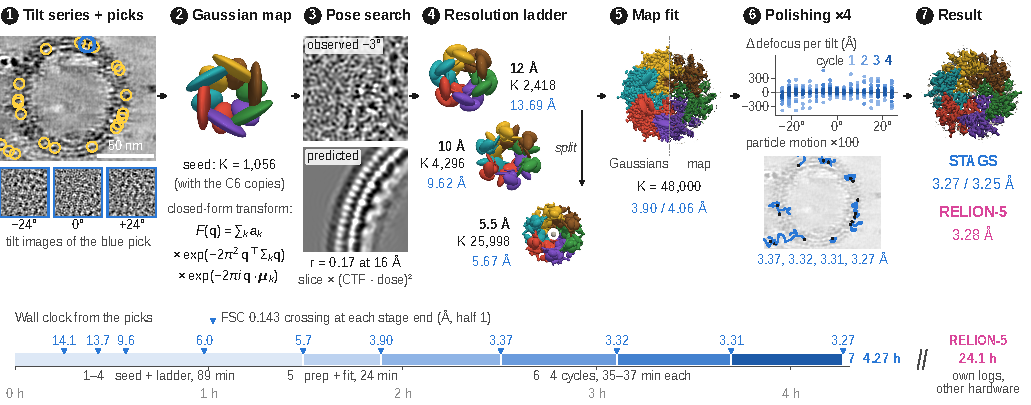
\includegraphics[width=\textwidth]{fig/teaser.pdf}
\captionsetup{hypcap=false}
\captionof{figure}{\textbf{STAGS step by step, on the final run (half-set~1; \cref{sec:method}).}
(1)~Initial picks (drawn on RELION's denoised tomogram, display only) give CTF-premultiplied tilt-image crops of each particle.
(2)~The map is a C6-symmetric mixture of anisotropic 3D Gaussians with a closed-form Fourier transform (seed model shown).
(3)~Candidate poses are scored on every tilt-image crop against the mixture's central slice times (CTF$\cdot$exposure filter)$^2$, the transfer of premultiplied crops (one tilt shown).
(4)~A resolution ladder alternates pose search and fitting, splitting Gaussians as resolution increases.
% src: kb/h1/fit0/B_4536_model.pt (8,000 Gaussians per asymmetric unit x 6 copies)
(5)~A fresh fit with $K=48{,}000$ Gaussians at the 5.5\,\AA\ poses: Gaussians (left) and the map they define (right).
% src: report.json cycles_minutes (4 cycles), stop rule in run_abc.log
(6)~Four polishing cycles re-estimate poses, per-tilt optics, tilt geometry and particle motion and refit the map; shown are each cycle's per-tilt defocus changes and particle tracks (magnified 100$\times$).
(7)~Final map (average of both halves), colored by subunit.
Bottom: wall clock from the picks; blue numbers are FSC~0.143 crossings against the opposite RELION-5 half map. RELION's time comes from its logs on other hardware.}
\captionsetup{hypcap=true}
\label{fig:teaser}%
\end{strip}
